\documentclass[11pt, oneside]{article} 
\usepackage{geometry}
\geometry{letterpaper} 
\usepackage{graphicx}
	
\usepackage{amssymb}
\usepackage{amsmath}
\usepackage{parskip}
\usepackage{color}
\usepackage{hyperref}

\graphicspath{{/Users/telliott_admin/Dropbox/Tex/png/}}
% \begin{center} 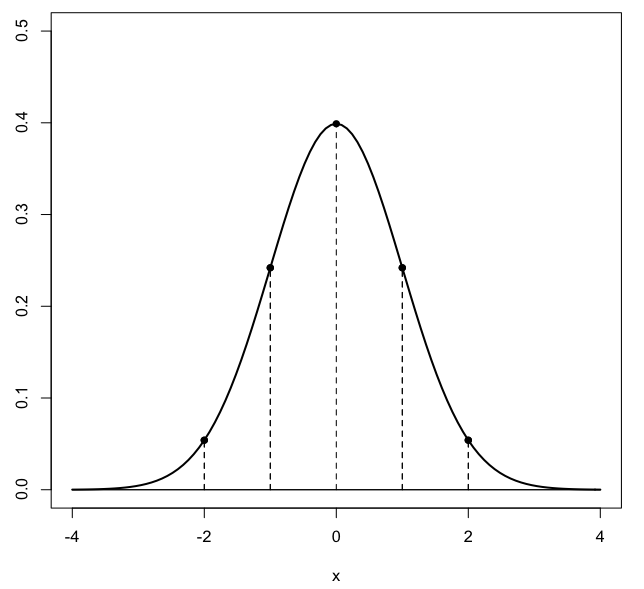
\includegraphics [scale=0.4] {gauss3.png} \end{center}

\title{Kepler:  Axes}
\date{}

\begin{document}
\maketitle
\Large

\begin{center} 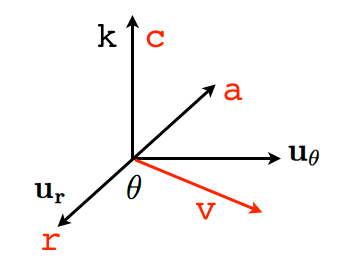
\includegraphics [scale=0.5] {Newton_vecs.png} \end{center}
Here is a sketch of the situation.  
$\mathbf{r}$ is the position vector, extending radially out from the sun to the planet.  $\mathbf{u_r}$ is a unit vector in the $\mathbf{r}$ direction, so that 
\[ \mathbf{r} = r \mathbf{u_r} \]

By the central force hypothesis, the acceleration $\mathbf{a} = \dot{\mathbf{v}} = \ddot{\mathbf{r}}$ is in the $- \mathbf{u_r}$ direction.  The source of all our complexity is that the velocity $\mathbf{v} = \dot{\mathbf{r}}$ is not perpendicular to $\mathbf{u_r}$ but makes an angle $\theta$ with it.

Earlier we proved that 
\[  \mathbf{r} \times \mathbf{v} = \mathbf{r} \times \dot{\mathbf{r}} = \mathbf{c} \]
is a constant.  Here we give that vector the label $\mathbf{c}$ and a direction.  We align $\mathbf{c}$ with $\hat{\mathbf{k}}$.  All the motion takes place in the $xy$-plane.  Finally, we define $\mathbf{u_{\theta}}$ as orthogonal to $\mathbf{u_{r}}$ (and to $\hat{\mathbf{k}}$).  $\mathbf{u_{\theta}}$ is aligned with $\hat{\mathbf{j}}$.

As a result of these definitions:  
\[ \mathbf{u_r} \times \mathbf{u_{\theta}} = \hat{\mathbf{k}} \]
\[ \hat{\mathbf{k}} \times \mathbf{u_r} = \mathbf{u_{\theta}} \]
\[ \mathbf{u_{\theta}} \times \hat{\mathbf{k}} = \mathbf{u_r} \]

At any given time, $\mathbf{r}$ makes an angle $\theta$ with the $x$-axis, and is at a distance $r$ from the origin, so we write:
\[ \mathbf{r} = \ \langle r \cos \theta, r \sin \theta, 0 \rangle = r \  \mathbf{u_r} \]
\[ \mathbf{u_r} =  \ \langle \cos \theta, \sin \theta, 0 \rangle \]

\[ \mathbf{u_{\theta}} \perp \mathbf{u_r} \]
\[ \mathbf{u_{\theta}} =  \ \langle -\sin \theta, \cos \theta, 0 \rangle \]
Verify that the dot-product is zero and that both vectors are unit length.

Now, differentiate $ \mathbf{u_r}$ and $\mathbf{u_{\theta}}$ (realizing that $\theta$ is also a function of time):
\[ \frac{d}{dt} \ \mathbf{u_r} = \dot{\mathbf{u}}_\mathbf{r} = \frac{d\theta}{dt} \ \langle -\sin \theta, \cos \theta, 0 \rangle = \ \frac{d\theta}{dt} \ \mathbf{u_{\theta}} \]

\[ \frac{d}{dt} \ \mathbf{u_{\theta}} = \dot{\mathbf{u}}_\mathbf{\theta} =  \frac{d\theta}{dt} \ \langle -\cos \theta, -\sin \theta, 0 \rangle = - \frac{d\theta}{dt} \ \mathbf{u_r} \]

Of course, with appropriate choice of units for time $t$, we can have $\theta = t$, so all of these factors of $d \theta/dt = 1$.

We can also get a parametric expression for the velocity
\[ \mathbf{v} = \dot{\mathbf{r}} = \frac{d}{dt} \ (r \mathbf{u_r}) = \frac{dr}{dt} \mathbf{u_r} + r \frac{d \theta}{dt}  \mathbf{u_{\theta}} \]

 and (with a little more work) we can get the acceleration
 \[ \mathbf{a} = \dot{\mathbf{v}} = \ddot{\mathbf{r}} = \frac{d}{dt} \ (\frac{dr}{dt} \mathbf{u_r} + r \frac{d \theta}{dt}  \mathbf{u_{\theta}}) \]
 \[ = \frac{d^2r}{dt^2} \mathbf{u_r} + \frac{dr}{dt} \dot{\mathbf{u}}_\mathbf{r} + \frac{dr}{dt} \frac{d \theta}{dt}  \mathbf{u_{\theta}} + r \frac{d^2\theta}{dt^2} \mathbf{u_{\theta}} + r \frac{d\theta}{dt} \dot{\mathbf{u}}_\mathbf{\theta}  \]
 
 We get three terms from differentiating the triple product $r \ d\theta/dt  \ \mathbf{u_{\theta}}$, by a variation on the product rule.  
 
 Substitute for the dotted terms from above
\[ = \frac{d^2r}{dt^2} \mathbf{u_r} + \frac{dr}{dt} \frac{d\theta}{dt} \ \mathbf{u_{\theta}} + \frac{dr}{dt} \frac{d \theta}{dt}  \mathbf{u_{\theta}} + r \frac{d^2\theta}{dt^2} \mathbf{u_{\theta}} - r \frac{d\theta}{dt} \frac{d\theta}{dt} \ \mathbf{u_r}  \]


Group common terms together
\[ = (\frac{d^2r}{dt^2} - r (\frac{d\theta}{dt})^2 ) \mathbf{u_r}  + (2 \ \frac{dr}{dt} \frac{d\theta}{dt} + r \frac{d^2\theta}{dt^2}) \mathbf{u_{\theta}}  \]

Now for a nice simplification, look at the factors multiplying $\mathbf{u_{\theta}}$ and recognize that
\[ \frac{d}{dt} ( r^2 \frac{d\theta}{dt}) = 2 r \frac{dr}{dt} \frac{d\theta}{dt} + r^2 \frac{d^2\theta}{dt^2}\]
Therefore, the cofactors for $\mathbf{u_{\theta}}$ can be re-written as
\[ \frac{1}{r} (\frac{d}{dt} ( r^2 \frac{d\theta}{dt}) \]

and since if the acceleration is to be only radial (pointed toward the sun), there is no torque and this term must be equal to zero.
\[ \frac{1}{r} (\frac{d}{dt} ( r^2 \frac{d\theta}{dt}) = 0 \]
\[ \frac{d}{dt} ( r^2 \frac{d\theta}{dt}) = 0 \]
\[ r^2 \frac{d\theta}{dt} = h = \text{constant} \]
If we write $d\theta/dt = \omega$, the angular velocity, then $r \omega$ is the speed of the planet, and $r$ times that, times the mass, is the angular momentum.  This result is the conservation of angular momentum.

\end{document}  